\Chapter{}
\chapter{MARCO TEÓRICO}
   \section{Antecedentes de la investigación}
        La armonización de imágenes de diferentes sensores es esencial para el monitoreo continuo y preciso de la superficie terrestre. En este contexto, un estudio en el 2019 abordó este desafío mediante la implementación de un marco de fusión basado en deep learning para mejorar la resolución espacial de las imágenes Landsat-8 utilizando imágenes Sentinel-2 como auxiliares. Los resultados cuantitativos del estudio mostraron que este enfoque, denominado ESRCNN, superó al algoritmo de referencia, el area-to-point regression kriging (ATPRK), en términos de precisión. En particular, para las imágenes del 15 de junio de 2017, el RMSE para la banda 1 fue de 0.0243, el coeficiente de correlación (CC) alcanzó valores de hasta 0.9860 y el Universal Image Quality Index (UIQI) registró valores de hasta 0.9710. Estos indicadores reflejan la alta eficacia del método propuesto en la preservación de la distribución de reflectancia de la imagen original y en la mejora de la resolución espacial. Estos hallazgos subrayan el potencial del deep learning en la armonización y recuperación de imágenes satelitales, lo que es relevante para investigaciones que buscan mejorar la calidad y consistencia de las series temporales de imágenes \autocite{shao2019deep}.

        Posteriormente, se llevó a cabo un estudio para entender mejor la relación entre las longitudes de onda reflectivas de Landsat-7 ETM+ y Landsat-8 OLI, y también para analizar la consistencia del Índice de Vegetación de Diferencia Normalizada (NDVI). Al analizar las trayectorias coincidentes, se examinaron 59 millones de observaciones de sensores de 30 m, obtenidas de 6317 imágenes. Los resultados mostraron que, en promedio, la reflectancia TOA de OLI supera a la de ETM+ en todas las bandas. Asimismo, en áreas con vegetación y terrenos, el NDVI de OLI tiende a ser superior al de ETM+. Para garantizar una transición fluida entre los datos de ambos, se introdujeron métodos estadísticos de transformación que mostraron un ajuste con coeficientes de determinación r2 de más de 0.7 para reflectancia y más de 0.9 para NDVI, con significancias estadísticas menores a 0.0001 \autocite{roy2016characterization}.
        
        Adicionalmente, en un estudio se aplicó el modelo ’ArithFusion’ basado en deep learning para fusionar imágenes de teledetección temporales multimodales. Esta investigación se centró en combinar imágenes de diferentes resoluciones y períodos de revisita, un aspecto crucial para la armonización efectiva de imágenes satelitales. El modelo propuesto, UMSEh, demostró ser eficaz, logrando un RMSE de 2.06 (0.57) en experimentos con escala 4x, lo que indica una alta precisión en la fusión de imágenes. Este estudio resalta el potencial del deep learning, como la arquitectura U-Net, en la armonización de imágenes satelitales, proporcionando una base sólida para futuras investigaciones en este campo \autocite{hoque2022arithfusion}. 
        
        Asimismo, una investigación llevada a cabo por \textcite{saunier2022sen2like} exploró la armonización y fusión de datos de sensores satelitales Landsat 8, Landsat 9 y Sentinel-2 utilizando técnicas avanzadas de inteligencia artificial. Mediante el software S2L, desarrollado en Python 3.7 e incorporando librerías como Numpy, Pandas y Scikit-Learn, se generaron conjuntos de datos armonizados (L2H) y fusionados (L2F). Estos conjuntos, tras meticulosos ajustes espectrales, se presentaron en mosaicos de 110 km × 110 km utilizando el Sistema de Referencia UTM-MGRS. Se aplicaron correcciones geométricas, apoyadas en herramientas como OpenCV, y se implementaron correcciones atmosféricas con la ayuda de SMAC y Sen2Cor 3.0. Uno de los avances más significativos fue la corrección BRDF, que logró reducir coeficientes hasta un 0.01◦. Además, se puso de manifiesto la variabilidad en respuestas espectrales entre diferentes instrumentos, llevando a la introducción del Factor de Ajuste de Banda Espectral (SBAF). La innovación de este estudio sirve como pilar para futuros esfuerzos enfocados en la integración y optimización de imágenes de diferentes sensores, estableciendo un precedente clave para trabajos que buscan la armonización en el monitoreo satelital.

        Recientemente, un avance importante se destacó en el campo de la super-resolución para teledetección, donde las redes generativas adversarias (GANs) han mostrado un potencial significativo en la producción de imágenes de super-resolución de alta fidelidad. La introducción de CLIPSCORE, una nueva métrica, ha mejorado notablemente la evaluación de las imágenes super-resueltas alineándose estrechamente con el juicio humano. Utilizando CLIPSCORE, las GANs demostraron ser superiores en comparación con métodos basados en pérdida L2 y mostraron una precisión semántica más alta que los modelos de difusión modernos. Este descubrimiento, apoyado en el uso del conjunto de datos S2-NAIP que abarca 113,000 km² con imágenes de Sentinel-2 y NAIP, facilita una investigación más profunda en este campo. La capacidad de las GANs para acelerar el entrenamiento hasta 18 veces, al tiempo que mejora la calidad de los resultados, subraya un avance crucial hacia la armonización eficaz y el monitoreo global, marcando un hito significativo en la aplicación de técnicas de inteligencia artificial en la teledetección \autocite{asdf}

    \section{Bases teóricas}
        \subsection{Armonización de imágenes satelitales}
            \subsubsection{Landsat: satélites de observación terrestre}
                Desde 1972, los satélites Landsat han adquirido de manera continua imágenes basadas en el espacio de la superficie terrestre de la Tierra. Estos datos son esenciales para investigaciones relacionadas con el uso y cambio del suelo, con aplicaciones en áreas como la silvicultura, agricultura, geología, planificación regional y educación.
                
                \paragraph{Historia y misión de Landsat}
                    Landsat es una colaboración entre el U.S. Geological Survey (USGS) y la National Aeronautics and Space Administration (NASA). Mientras NASA se encarga del desarrollo de los instrumentos y satélites, así como de su lanzamiento y validación, el USGS toma control sobre la operación de los satélites, la recepción de datos, archivo, generación de productos y distribución \autocite{USGS2023}.
                    
                    % \insertfigure
                    %     {Línea de tiempo e historia de las misiones Landsat, iniciadas en 1972.}
                    %     {2_CAPITULO0/IMG/linea_tiempo_landsat.png}
                    %     {La línea de tiempo destaca que, desde su inicio en 1972, las misiones Landsat han brindado una secuencia constante de datos que revelan las transformaciones de la Tierra, apoyando así diversas investigaciones y evidenciando su desarrollo en la vigilancia ambiental global. Tomado de \textcite{USGS2023}.} 


                    \begin{figure}[H] 
                        \caption{\doublespacing \\ \textit{Línea de tiempo e historia de las misiones Landsat, iniciadas en 1972.}} 
                        \centering
                        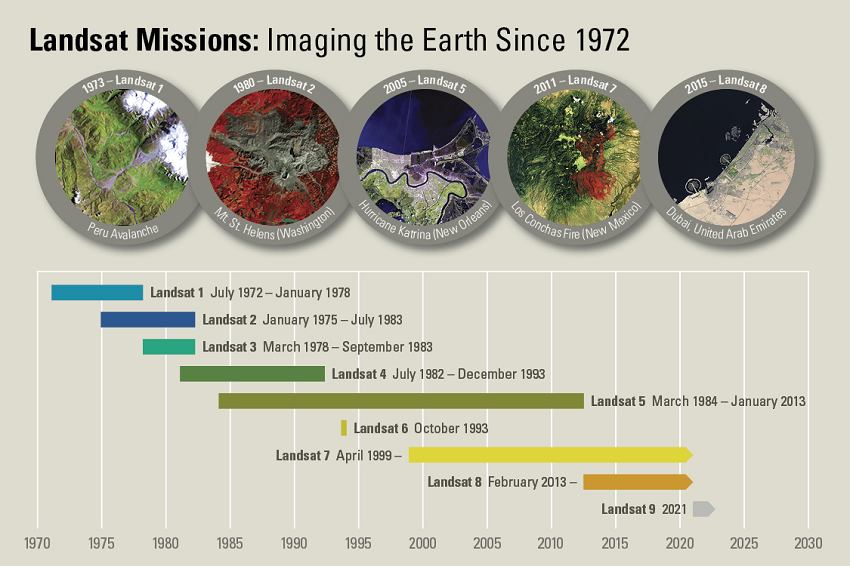
\includegraphics[width=1\linewidth]{2_CAPITULO0/IMG/linea_tiempo_landsat.png}
                        \begin{justify}
                            \textit{Nota.} La línea de tiempo destaca que, desde su inicio en 1972, las misiones Landsat han brindado una secuencia constante de datos que revelan las transformaciones de la Tierra, apoyando así diversas investigaciones y evidenciando su desarrollo en la vigilancia ambiental global. Tomado de \textcite{USGS2023}.
                        \end{justify}                    
                        \label{landsat_missions}
                    \end{figure}



                    La idea de crear un satélite de observación civil surgió en la década de 1960, lográndose el 23 de julio de 1972 con el lanzamiento de ERTS-1, luego renombrado Landsat 1. A este le siguieron varias versiones, siendo Landsat 5 el que estableció un récord por ser el satélite de observación terrestre en funcionamiento más longevo.
                
                \paragraph{Adquisiciones satelitales}
                    Tanto Landsat 8 como Landsat 9 orbitan la Tierra a una altitud de 705 km, completando una órbita en 99 minutos y pasando por cualquier punto de la Tierra cada 16 días. Entre los dos satélites, se agregan más de 1,500 escenas al archivo USGS diariamente. Landsats 4, 5 y 7 siguieron la misma órbita, mientras que Landsats 1, 2 y 3 tenían una altitud de 920 km \autocite{USGS2023}.
                
                \paragraph{Sensores y designaciones de bandas}
                    Los sensores han variado a lo largo de las versiones de Landsat. Desde el Multispectral Scanner (MSS) en los primeros Landsats hasta el Operational Land Imager (OLI) y el Thermal Infrared Sensor (TIRS) en los Landsats más recientes.
                
                    \begin{table}[H]
                        \caption{\doublespacing \\ \textit{Comparación y visualización de bandas y longitudes de onda de sensores Landsat mediante Spectral Viewer del U.S. Geological Survey.}}
                        \begin{spacing}{8}
                            \fontsize{8pt}{2pt}\selectfont  
                            \begin{tabularx}{\linewidth}{P{3cm}*{10}{c}} 
                                \toprule
                                \textbf{Designaciones de banda} & \multicolumn{2}{c}{\textbf{L8-9 OLI/TIRS}} & \multicolumn{2}{c}{\textbf{L7 ETM+}} & \multicolumn{2}{c}{\textbf{L4-5 TM}} & \multicolumn{2}{c}{\textbf{L4-5 MSS*}} & \multicolumn{2}{c}{\textbf{L1-3 MSS*}} \\
                                \midrule
                                & B & Longitud & B & Longitud & B & Longitud & B & Longitud & B & Longitud \\
                                \midrule
                                Costera/Aerosol & 1 & 0.43–0.45 & -- & -- & -- & -- & -- & -- & -- & -- \\
                                Azul & 2 & 0.45–0.51 & 1 & 0.45–0.52 & 1 & 0.45–0.52 & -- & -- & -- & -- \\
                                Verde & 3 & 0.53–0.59 & 2 & 0.52–0.60 & 2 & 0.52–0.60 & 1 & 0.5–0.6 & 4 & 0.5–0.6 \\
                                Pancromática** & 8  & 0.50–0.68 & 8 & 0.52–0.90 & -- & -- & -- & -- & -- & -- \\
                                Rojo & 4 & 0.64–0.67 & 3 & 0.63–0.69 & 3 & 0.63–0.69 & 2 & 0.6–0.7 & 5 & 0.6–0.7 \\
                                Infrarrojo cercano & 5 & 0.85–0.88 & 4 & 0.77–0.90 & 4 & 0.76–0.90 & 3 & 0.7–0.8 & 6 & 0.7–0.8 \\
                                Infrarrojo cercano & -- & -- & -- & -- & -- & -- & 4 & 0.8–1.1 & 7 & 0.8–1.1 \\
                                Cirrus & 9 & 1.36–1.38 & -- & -- & -- & -- & -- & -- & -- & -- \\
                                Infrarrojo corto-1 & 6 & 1.57–1.65 & 5 & 1.55–1.75 & 5 & 1.55–1.75 & -- & -- & -- & -- \\
                                Infrarrojo corto-2 & 7 & 2.11–2.29 & 7 & 2.09–2.35 & 7 & 2.08–2.35 & -- & -- & -- & -- \\
                                Térmico & 10 T1 & 10.60–11.19 & 6 T2 & 10.40–12.50 & 6 T2 & 10.40–12.50 & -- & -- & -- & -- \\
                                Térmico & 11 T1 & 11.50–12.51 & -- & -- & -- & -- & -- & -- & -- & -- \\
                                \bottomrule
                            \end{tabularx}
                        \end{spacing}
                        \vspace{1\baselineskip}
                        \textit{Nota.} Hay observaciones que se debe tener en cuenta. Adapatado de \textcite{Landsat2023}. \\
                            * Adquirido a 80 metros, remuestreado a 60 metros. \\
                            ** 15 metros (pancromático). \\
                            T1 = Térmico (adquirido a 100 metros, remuestreado a 30 metros). \\
                            T2 = Térmico (adquirido a 120 metros, remuestreado a 30 metros). 
                        \label{BandasLandsat}
                    \end{table}
                
                    \begin{table}[H]
                        \caption{\doublespacing \\ \textit{Comparación de sensores Landsat}}
                        \begin{spacing}{8}
                            \fontsize{8pt}{2pt}\selectfont  
                            \begin{tabularx}{\linewidth}{*{6}{c}P{3.5cm}} 
                                \toprule
                                \textbf{Banda} & \textbf{L8–9 OLI/TIRS} & \textbf{L7 ETM+} & \textbf{L4–5 TM} & \textbf{L4–5 MSS} & \textbf{L1–3 MSS} & \multicolumn{1}{c}{\textbf{Uso}} \\
                                \midrule
                                Costero/Aerosol & Banda 1 & -- & -- & -- & -- & Observaciones costeras y detección de aerosoles. \\
                                Azul & Banda 2 & Banda 1 & Banda 1 & -- & -- & Mapeo batimétrico y discriminación suelo/vegetación. \\
                                Verde & Banda 3 & Banda 2 & Banda 2 & Banda 1 & Banda 4 & Evaluación de la vegetación. \\
                                Rojo & Banda 4 & Banda 3 & Banda 3 & Banda 2 & Banda 5 & Identificación de vegetación y suelos. \\
                                Infrarrojo Cercano & Banda 5 & Banda 4 & Banda 4 & Banda 3 & Banda 6 & Análisis y detección de vegetación. \\
                                & -- & -- & -- & Banda 4 & Banda 7 &  \\
                                Infrarrojo Onda Corta-1 & Banda 6 & Banda 5 & Banda 5 & -- & -- & Análisis de humedad y detección de incendios. \\
                                Infrarrojo Onda Corta-2 & Banda 7 & Banda 7 & Banda 7 & -- & -- & Detección de incendios y análisis de humedad. \\
                                Panchromático & Banda 8 & Banda 8 & -- & -- & -- & Mejora de resolución en imágenes multiespectrales. \\
                                Cirrus & Banda 9 & -- & -- & -- & -- & Detección de nubes cirrus. \\
                                Térmico & Banda 10 & Banda 6 & Banda 6 & -- & -- & Mapeo de temperatura y estimación de humedad.
                                \\
                                \bottomrule
                            \end{tabularx}
                        \end{spacing}
                        \vspace{1\baselineskip}
                        \textit{Nota.} Se observa una tendencia en el uso de diferentes bandas para monitorear vegetación, analizar humedad, clima y mejorar la resolución de imágenes. Adaptado de \textcite{Landsat2023}.
                        \label{UsoLandsat}
                    \end{table}
                
                \paragraph{Aplicaciones de los datos Landsat}
                    Los datos de Landsat respaldan una amplia gama de aplicaciones, desde investigación del cambio global hasta seguimiento de derrames de petróleo y monitoreo de contaminación por residuos mineros.
                    

            \subsubsection{Landsat MSS}
                El Multispectral Scanner (MSS) fue el primer sensor de Landsat, utilizado en las misiones Landsat 1 a 5. Este sensor capturaba imágenes en cuatro bandas espectrales, con una resolución espacial de 79 metros para las bandas 1 a 4 y de 185 metros para la banda 5. Aunque el MSS fue reemplazado por el Thematic Mapper (TM) en Landsat 4, 5 y 7, sus datos siguen siendo valiosos para estudios de largo plazo y análisis de series temporales \autocite{landsat_legacy}.
                \paragraph{Landsat 1 (ERTS-1) y su MSS}
                    Originalmente denominado Earth Resources Technology Satellite (ERTS-1), fue lanzado el 23 de julio de 1972. El satélite llevaba a bordo el MSS, un sistema de escaneo multiespectral que capturaba imágenes en cuatro bandas espectrales (verde, rojo, y dos infrarrojas cercanas) con una resolución espacial de 80 metros . Esta tecnología permitía detectar y analizar cambios en el uso del suelo y la vegetación con mayor detalle que los sistemas anteriores.
                    Durante su operación, Landsat 1 experimentó problemas técnicos, como la falla de una de sus grabadoras de cinta de video en agosto de 1972, seguida por la segunda en 1974, lo que limitó la capacidad de grabar datos de manera continua . A pesar de estos desafíos, el MSS proporcionó imágenes claras y precisas que demostraron ser esenciales para una variedad de aplicaciones científicas y de gestión de recursos.

                    \begin{figure}[H] 
                        \caption{\doublespacing \\ \textit{Primera imagen terrestre sin nubes adquirida por el Landsat 1 MSS, 25 de julio de 1972.}} 
                        \centering
                        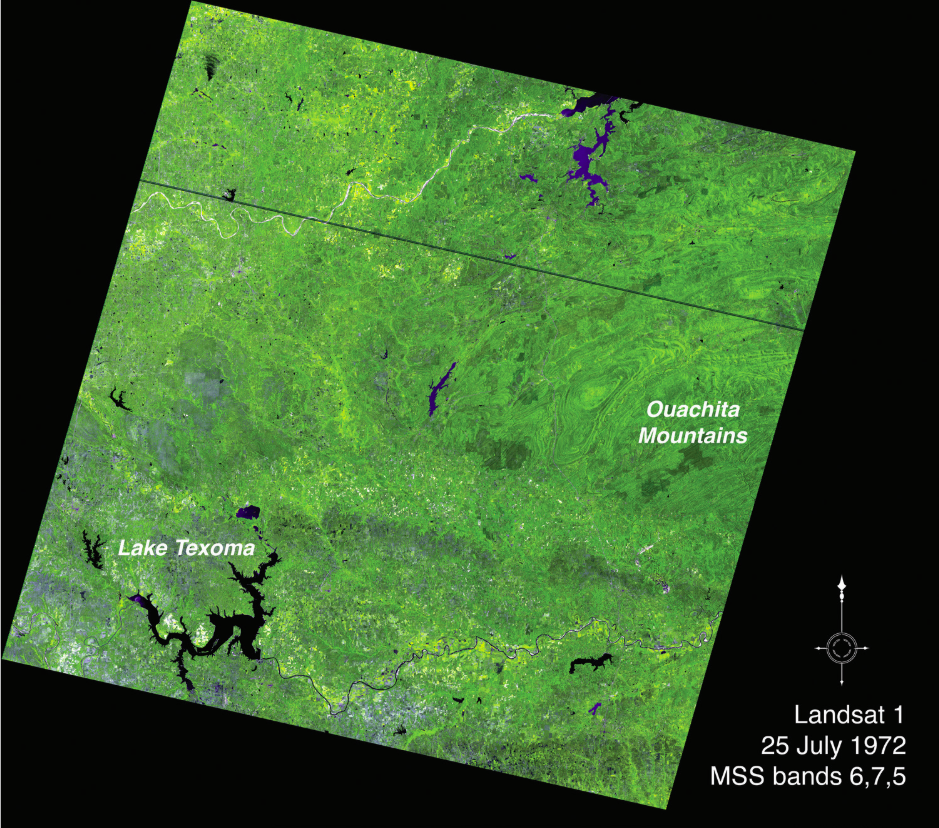
\includegraphics[width=1\linewidth]{2_CAPITULO2/IMG/landsat1.png}
                        \begin{justify}
                            \textit{Nota.} Imagen sin nubes del sistema MSS de Landsat 1 mostrando las Montañas Ouachita en el sureste de Oklahoma. Tomado de \textcite{landsat_legacy}.
                        \end{justify}                    
                        \label{landsat1}
                    \end{figure}

                \paragraph{Landsat 2}
                    Lanzado el 22 de enero de 1975, fue diseñado de manera similar a Landsat 1 y continuó la misión de su predecesor con mejoras en la recopilación y manejo de datos . Landsat 2 también estaba equipado con el MSS, que siguió siendo el instrumento principal para la recolección de datos. A lo largo de su misión, Landsat 2 recopiló una vasta cantidad de datos MSS, aunque enfrentó problemas similares con sus grabadoras de cinta, lo que eventualmente afectó su capacidad operativa.

                    \begin{figure}[H] 
                        \caption{\doublespacing \\ \textit{Fondos de escenas de USGS EROS MSS archivados en 1975 por Landsat 1 y Landsat 2.}} 
                        \centering
                        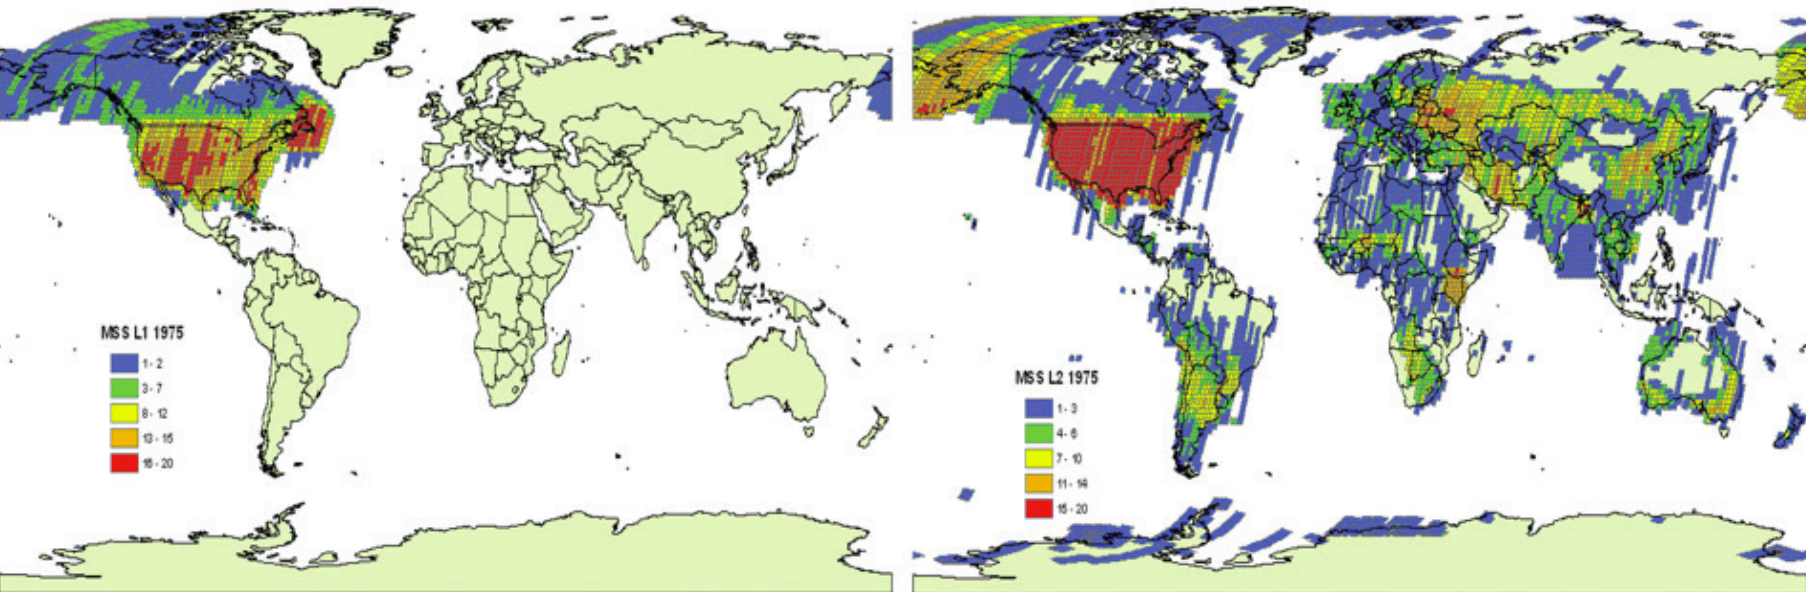
\includegraphics[width=1\linewidth]{2_CAPITULO2/IMG/landsat2.png}
                        \begin{justify}
                            \textit{Nota.} Comparación de las escenas MSS archivadas de Landsat 1 y 2 en 1975, mostrando la cantidad y distribución de datos recopilados. Tomado de \textcite{landsat_legacy}.
                        \end{justify}                    
                        \label{landsat2}
                    \end{figure}

                \paragraph{Landsat 3}
                    Lanzado el 5 de marzo de 1978, introdujo algunas mejoras en el MSS, incluyendo una banda infrarroja térmica para la recolección de datos nocturnos . Sin embargo, el satélite enfrentó varios problemas técnicos que afectaron su rendimiento. La calidad de los componentes del MSS era inferior a la de los satélites anteriores, lo que resultó en fallas recurrentes y una disminución en la calidad de los datos . A pesar de estos problemas, Landsat 3 contribuyó con valiosos datos MSS hasta su retiro en 1983.
                    
                    \begin{figure}[H] 
                        \caption{\doublespacing \\ \textit{Inicio de los problemas de inicio de línea Landsat 3 MSS.}} 
                        \centering
                        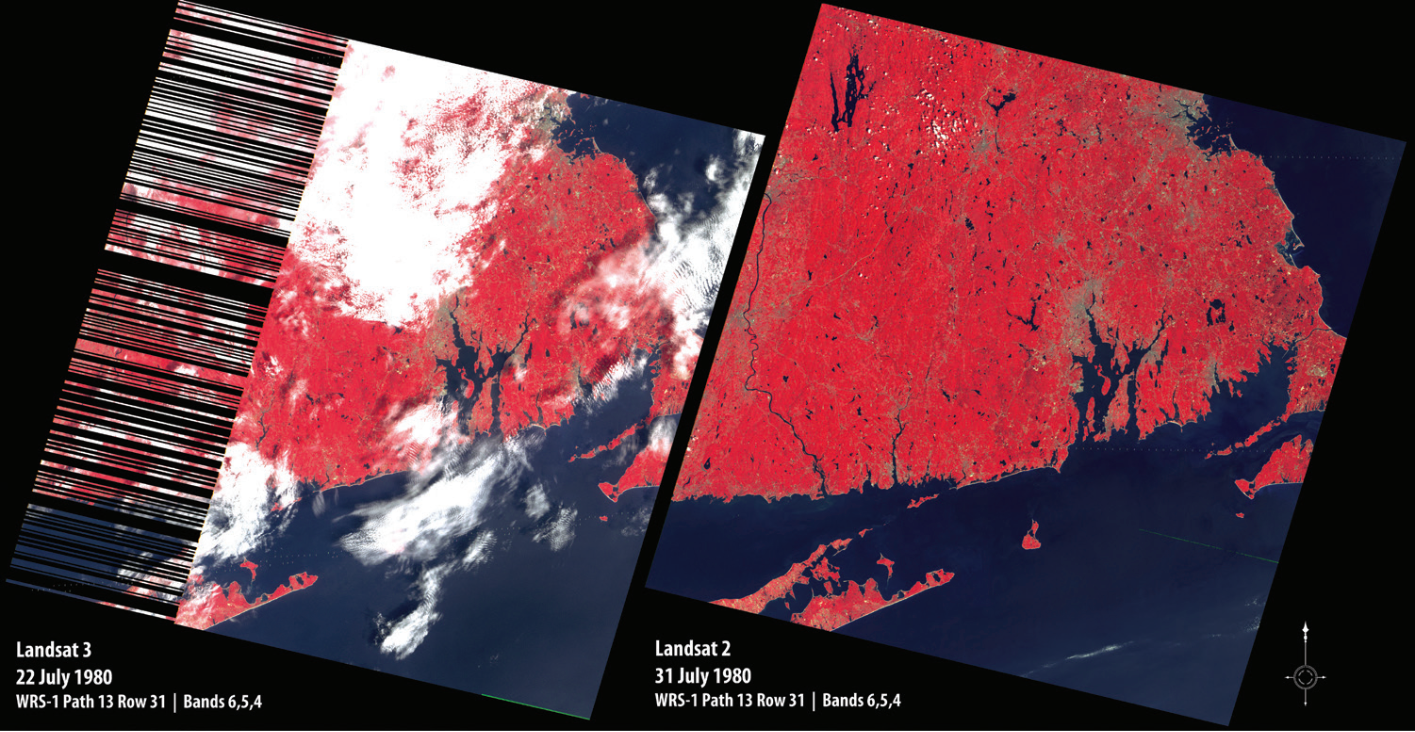
\includegraphics[width=1\linewidth]{2_CAPITULO2/IMG/landsat3.png}
                        \begin{justify}
                            \textit{Nota.} Imagen que muestra los problemas de inicio de línea del MSS de Landsat 3 en comparación con una imagen MSS de Landsat 2. Tomado de \textcite{landsat_legacy}.
                        \end{justify}                    
                        \label{landsat3}
                    \end{figure}

                \paragraph{Landsat 4}
                    Lanzado el 16 de julio de 1982, marcó una evolución significativa con la introducción del Thematic Mapper (TM), aunque el MSS continuó operando como un sensor secundario​​ . Landsat 4 enfrentó desafíos técnicos con su sistema de transmisión de datos, lo que limitó inicialmente la cantidad de datos MSS que pudo recolectar. No obstante, cuando la capacidad de transmisión se estabilizó, Landsat 4 proporcionó una cobertura casi completa a través de TDRS (Tracking and Data Relay Satellite) hasta 1987.

                    \begin{figure}[H] 
                        \caption{\doublespacing \\ \textit{Mapas de cobertura anual de Landsat 4 MSS (1982-1992).}} 
                        \centering
                        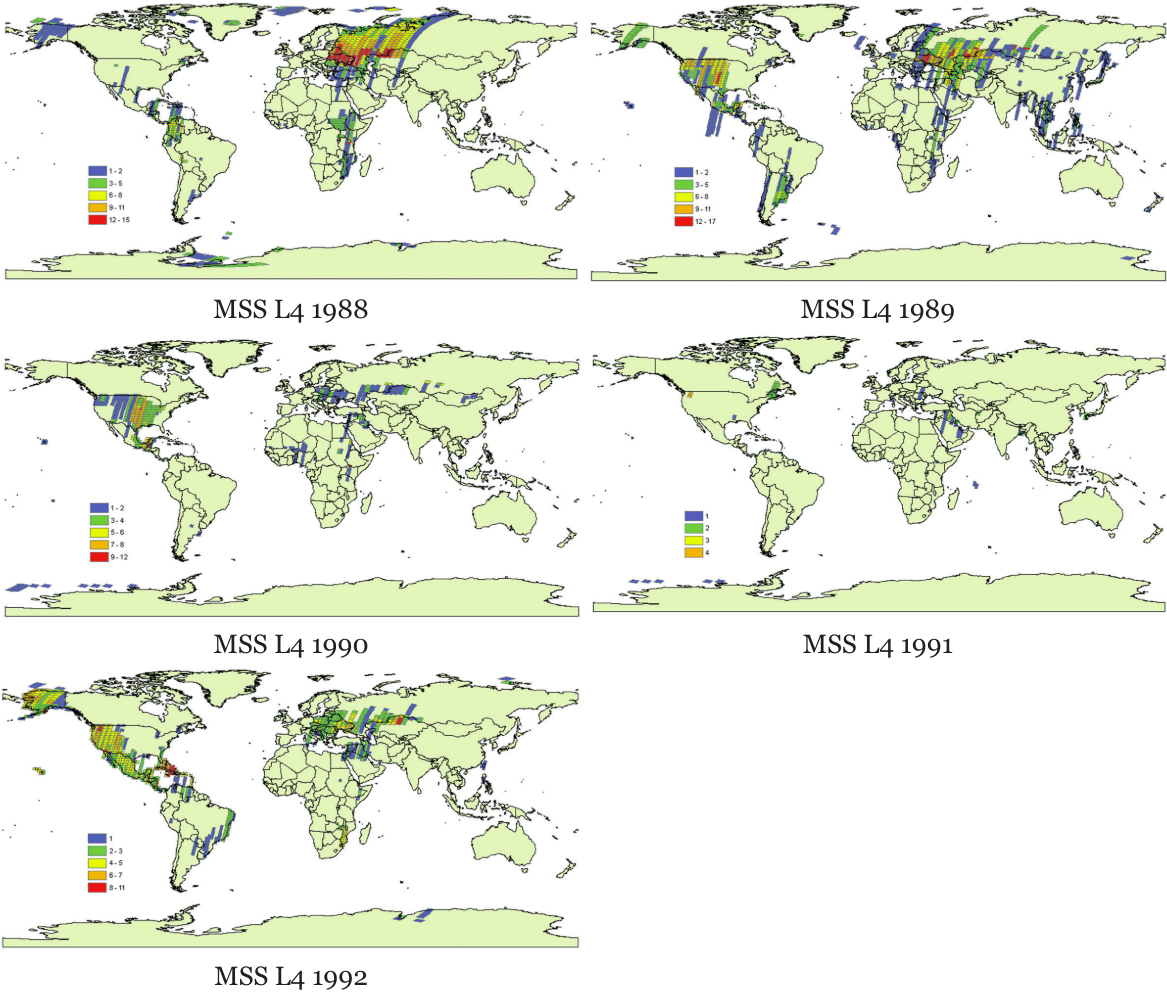
\includegraphics[width=1\linewidth]{2_CAPITULO2/IMG/landsat4.png}
                        \begin{justify}
                            \textit{Nota.} Mapas de cobertura anual del MSS de Landsat 4, mostrando la cobertura geográfica durante su operación. Tomado de \textcite{landsat_legacy}.
                        \end{justify}                    
                        \label{landsat4}
                    \end{figure}

                \paragraph{Landsat 5}
                    Lanzado el 1 de marzo de 1984, es conocido por su longevidad, operando mucho más allá de su vida útil diseñada . Al igual que Landsat 4, Landsat 5 estaba equipado tanto con el TM como con el MSS. Aunque el MSS dejó de ser el sensor principal, continuó recolectando datos valiosos hasta mediados de la década de 1990. Landsat 5 es reconocido por el Guinness World Records como el satélite de observación de la Tierra más duradero en la historia.

                    \begin{figure}[H] 
                        \caption{\doublespacing \\ \textit{Mapas de cobertura anual de Landsat 5 MSS (1984-2007).}} 
                        \centering
                        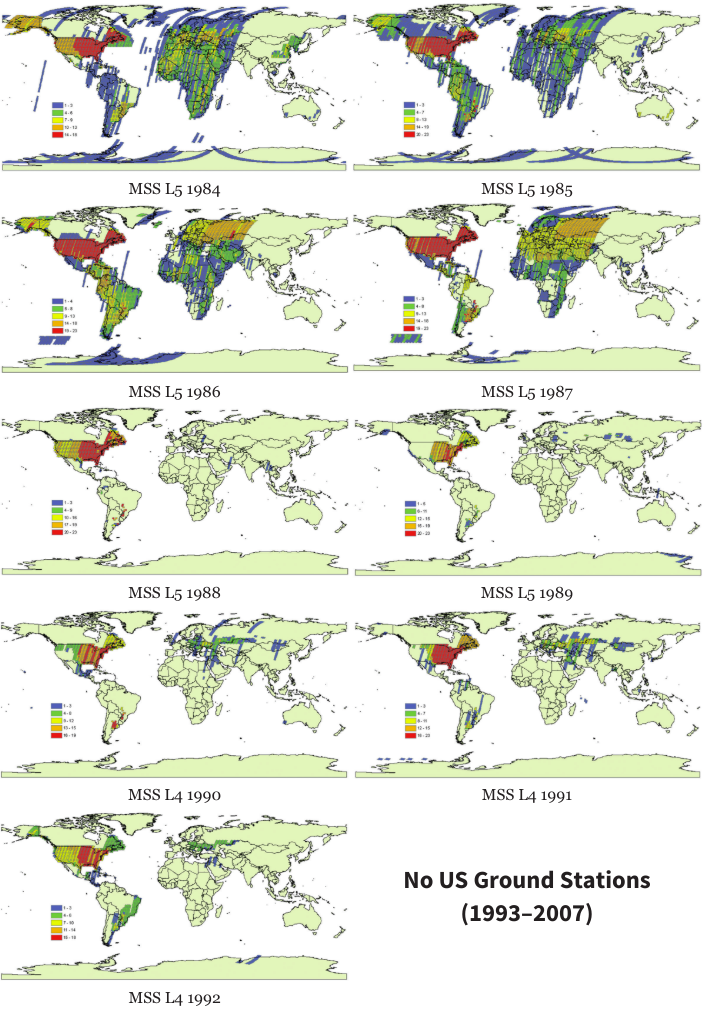
\includegraphics[width=0.9\linewidth]{2_CAPITULO2/IMG/landsat5.png}
                        \begin{justify}
                            \textit{Nota.} Mapas de cobertura anual del MSS de Landsat 5, mostrando la cobertura geográfica durante su operación. Tomado de \textcite{landsat_legacy}.
                        \end{justify}                    
                        \label{landsat5}
                    \end{figure}

                \paragraph{Fechas del Landsat MSS}
                    Las fechas operativas de los sensores MSS de Landsat pueden parecer confusas debido a las múltiples fases de operación y reactivación. El sensor MSS del Landsat cubrió el período desde 1972 hasta 1999, reflejando el uso operativo en los satélites Landsat 1 hasta Landsat 5. En el caso del Landsat 5 MSS, estuvo operativo hasta 2012 porque, aunque dejó de ser la carga principal a finales de los años 90, se reactivó temporalmente en 2012 para llenar brechas de datos antes de la desactivación final del satélite. La reactivación en 2012 se debió a la suspensión de la recopilación de datos TM a finales de 2011, lo que llevó a la reanudación rutinaria de la adquisición MSS hasta diciembre de 2012.

            \subsubsection{Landsat TM}
                El Landsat Thematic Mapper (TM) es un sensor clave en la historia de la observación de la Tierra, destacándose por sus mejoras significativas en resolución espacial y espectral en comparación con sus predecesores. Diseñado para captar imágenes multiespectrales, el TM está equipado con bandas espectrales que cubren desde el azul hasta el infrarrojo térmico, permitiendo una amplia gama de aplicaciones en monitoreo ambiental, gestión de recursos naturales y estudios científicos \autocite{landsat_legacy}.

                \paragraph{Landsat 4}
                    Fue lanzado el 16 de julio de 1982, representando un avance significativo en la teledetección debido a la inclusión del sensor Thematic Mapper (TM). A pesar de sus innovaciones, Landsat 4 enfrentó varios desafíos operacionales desde el inicio, incluyendo fallos en los transmisores de banda X, lo que limitó la capacidad de transmisión de datos del TM hasta que se estableció una conexión a través del sistema de satélites de retransmisión de datos (TDRSS).
                    
                    - \textbf{Problemas de comunicación:} Poco después del lanzamiento, Landsat 4 experimentó fallos en sus transmisores de banda X, dificultando la transmisión de imágenes TM. El lanzamiento del satélite TDRS-E permitió eventualmente la transmisión de datos del TM, aunque con cobertura limitada.
                    
                    - \textbf{Fallos en paneles solares:} En 1983, Landsat 4 perdió el 50\% de su capacidad de generación de energía debido a fallos en los paneles solares. Este problema limitó las operaciones del satélite, afectando su capacidad de recopilación de datos.

                    \begin{figure}[H] 
                        \caption{\doublespacing \\ \textit{Imagen de prueba del Thematic Mapper descargada vía TDRS-E el 12 de agosto de 1983.}} 
                        \centering
                        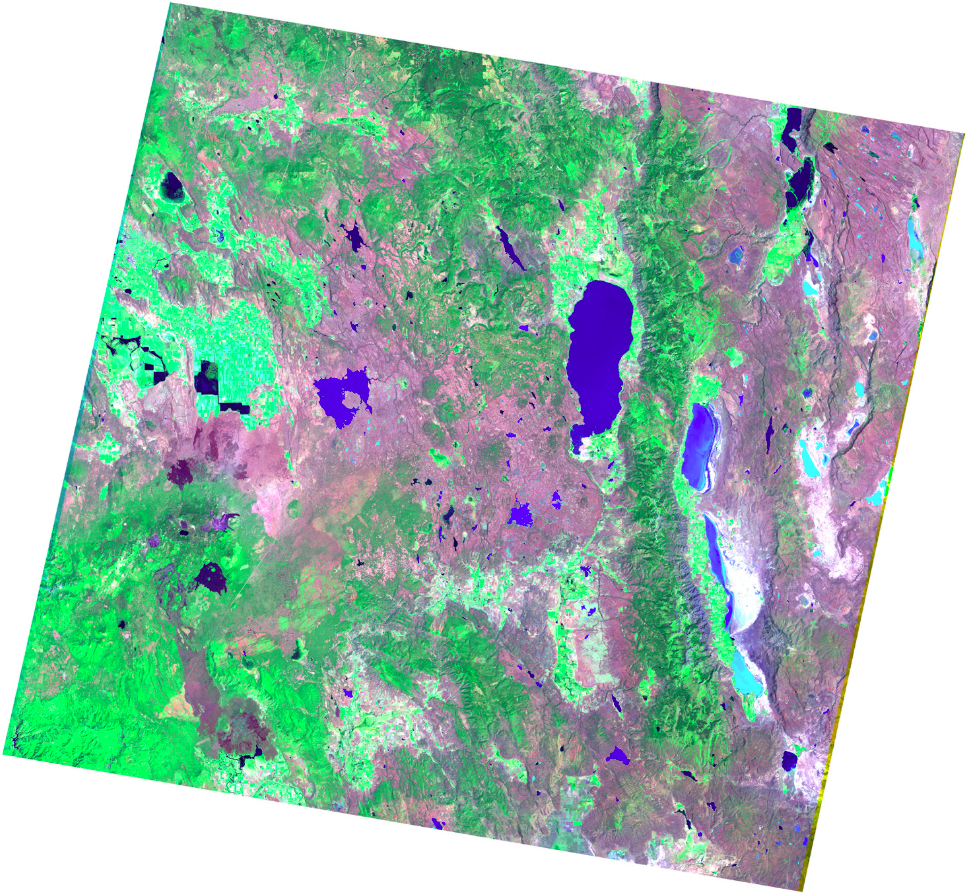
\includegraphics[width=1\linewidth]{2_CAPITULO2/IMG/landsat4_tm.png}
                        \begin{justify}
                            \textit{Nota.} Se muestra un área alrededor de la frontera California/Oregón, incluyendo Goose Lake, Clear Lake National Refuge, Lava Beds National Monument y Modoc National Forest (TM Bandas 7, 4, 2​). Tomado de \textcite{landsat_legacy}.
                        \end{justify}                    
                        \label{landsat4_tm}
                    \end{figure}

                \paragraph{Landsat 5}
                    Fue lanzado el 1 de marzo de 1984, y se destacó por su longevidad operativa, superando significativamente su vida útil de diseño inicial de tres años. Este satélite continuó recopilando datos hasta 2013, estableciendo un récord como la misión satelital de observación de la Tierra más duradera.

                    - \textbf{Desempeño del TM:} A lo largo de su misión, Landsat 5 proporcionó datos de alta calidad gracias al sensor TM, a pesar de enfrentar problemas de comunicación y fallos técnicos. La redundancia en los sistemas críticos y una mayor capacidad de combustible contribuyeron a su longevidad.

                    - \textbf{Innovaciones y aplicaciones:} Las mejoras en resolución espectral y radiométrica del TM permitieron aplicaciones avanzadas en clasificación de tierras y monitoreo ambiental. Estudios realizados con los datos del TM demostraron mejoras significativas en la precisión de clasificación, aunque la resolución espacial mejorada del TM no siempre resultó en mejoras proporcionales en todas las aplicaciones.

                    \begin{figure}[H] 
                        \caption{\doublespacing \\ \textit{Sub-sección de una de las primeras imágenes registradas por el Thematic Mapper de Landsat 5.}} 
                        \centering
                        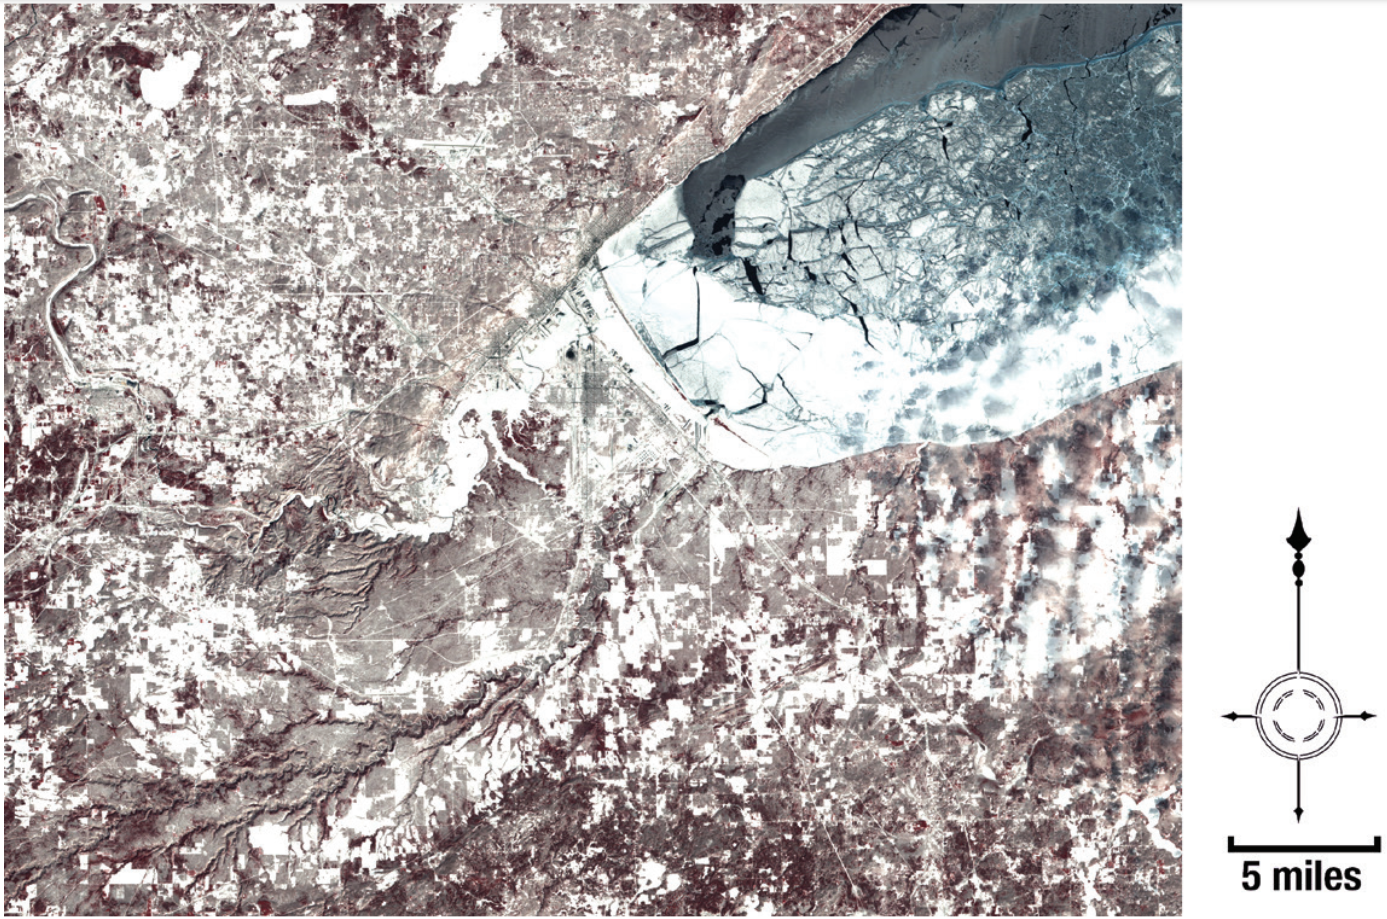
\includegraphics[width=1\linewidth]{2_CAPITULO2/IMG/landsat5_tm.png}
                        \begin{justify}
                            \textit{Nota.} Se muestra Duluth, Minnesota y el rompimiento del hielo en el Lago Superior, adquirida el 6 de marzo de 1984​. Tomado de \textcite{landsat_legacy}.
                        \end{justify}                     
                        \label{landsat5_tm}
                    \end{figure}

            \subsubsection{Armonización de imágenes en Teledetección}
                La armonización se refiere al ajuste radiométrico y geométrico de imágenes de múltiples sensores para garantizar la confiabilidad en teledetección \autocite{ichikawa2022development}. A medida que aumenta la disponibilidad de datos de teledetección, es esencial normalizar imágenes con propiedades radiométricas variables para mosaicos coherentes \autocite{langheinrich2017enhanced}. Además, implica alinear datos de diferentes fuentes para interpretaciones uniformes, utilizando modelos específicos como Fiware \autocite{vosinakis2022data}. Sin embargo, al estudiar la temperatura de la superficie terrestre, la armonización enfrenta desafíos debido a sesgos entre diferentes satélites \autocite{adeniran2022cross}.
                
            \subsubsection{Armonización geométrica de datos de Teledetección}
                Los datos de teledetección a menudo presentan desafíos inherentes. Uno de los principales es la falta de alineación perfecta entre imágenes, lo que da lugar a lo que se conoce como desajustes espaciales o misregistrations \autocite{storey2016note, wolfe2002achieving, yan2018sentinel}. Estos desajustes pueden oscilar desde sub-píxeles hasta unos pocos píxeles.
                
                \paragraph{Causas de desalineaciones}
                    Estos desajustes pueden ser atribuidos a diversas causas, desde la densidad desigual de puntos de control en tierra, el uso de conjuntos de datos de referencia desiguales, hasta problemas en el software de preprocesamiento de los proveedores o movimientos no modelados del sensor \autocite{storey2016note}. Estos desajustes, si no se corrigen, pueden afectar gravemente productos derivados, como clasificaciones de imágenes y detección de cambios.
                    
                \paragraph{Proceso de armonización}
                    La armonización geométrica tiene como objetivo abordar y corregir estas heterogeneidades espaciales. Se compone de dos fases principales: (1) la corrección de misregistrations, y (2) el remuestreo y reproyección de los datos \autocite{roy2000impact}. Sin embargo, corregir estos desajustes no es una tarea sencilla. Las imágenes pueden haber sido adquiridas en diferentes ángulos, fechas, y horarios, lo que complica aún más el proceso de armonización.
                    
                \paragraph{Resampling y Pan-sharpening}
                    A pesar de los desafíos, se han desarrollado técnicas para adaptar diferentes cuadrículas de píxeles mediante remuestreo espacial o pan-sharpening \autocite{ghassemian2016review, javan2021review, li2017pixel}. Estas técnicas están implementadas en varios paquetes de software de código abierto.
                    
                \paragraph{Técnicas de co-registración}
                    Las técnicas de co-registración son esenciales para alinear correctamente las imágenes. Estas técnicas se pueden clasificar en dos categorías principales: basadas en características y basadas en intensidad \autocite{zitova2003image}. Mientras que las primeras se centran en características notables en las imágenes, como edificios o carreteras, las segundas se basan en patrones de valores de grises. Ambas técnicas ofrecen sus propios beneficios y desafíos. 
                    
                \paragraph{Necesidad de un método universal}
                    Dada la diversidad y complejidad de los datos de teledetección, es esencial contar con un método de co-registración que sea universalmente aplicable \autocite{chen2003mutual}. Este método debería ser capaz de manejar desajustes técnicos entre múltiples sensores y desafíos presentados por paisajes y atmósferas cambiantes.

            \subsubsection{Armonización espectral de datos de Teledetección}
                Los sensores de teledetección óptica se caracterizan por presentar diversos bandas espectrales, abarcando no solo el espectro electromagnético visible (VIS, ~400 – 700 nm), sino también el infrarrojo cercano (NIR, ~750 – 1000 nm) y el infrarrojo de onda corta (SWIR, ~1000 – 2500 nm). Estos sensores facilitan la diferenciación de materiales superficiales y permiten identificar ciertas propiedades del cobertura terrestre o composiciones atmosféricas.
                
                \paragraph{Discrepancias espectrales entre sensores}
                    Aunque satélites de Observación de la Tierra (EO) como Landsat (NASA) o Sentinel-2 (ESA) suelen diseñarse con características espectrales similares para garantizar la comparabilidad a largo plazo, aún existen discrepancias en el número de bandas y las respuestas espectrales de cada sensor \autocite{drusch2012sentinel}.
                    
                \paragraph{Objetivo de la armonización espectral}
                    La armonización espectral busca transformar la información espectral de un sensor al dominio espectral de otro, con el fin de estandarizar el número de bandas y reducir inconsistencias entre imágenes de múltiples sensores, facilitando así análisis y flujos de trabajo posteriores.
                    
                \paragraph{Técnicas existentes}
                    Existen técnicas basadas en relaciones estadísticas de bandas equivalentes de múltiples sensores para lograr una transformación espectral \autocite{chastain2019empirical, claverie2018harmonized, flood2014continuity, roy2016characterization}. Sin embargo, estas técnicas están limitadas a bandas con equivalentes directos entre sensores, lo que deja un potencial no aprovechado en regiones espectrales como el borde rojo \autocite{filella1994red}.
                    
                \paragraph{Necesidad de avances metodológicos}
                    Es fundamental avanzar en las técnicas existentes de armonización espectral para estimar con precisión la información espectral faltante y reducir los errores de armonización que varían espacialmente. Además, es esencial evaluar el rendimiento de diferentes técnicas de armonización y cuantificar los errores de estimación según los materiales superficiales y las longitudes de onda de las bandas estimadas.
                    
            \subsubsection{Normalización y ajuste de datos con aplicación de parámetros BRDF}    

                \paragraph{Fundamentos de la función de distribución bidireccional de reflectancia (BRDF)}
                    En estudios anteriores, la BRDF se estableció como una función esencial que caracteriza cómo la luz es reflejada por las superficies terrestres en varias direcciones. Se observó que las superficies no son Lambertianas, lo que significa que la reflectancia varía con la geometría solar y de observación. Esto es crucial para corregir y comparar datos de reflectancia obtenidos en diferentes momentos y bajo diversas condiciones de iluminación \autocite{roy2016general}.
                \paragraph{Aplicación de parámetros BRDF en la normalización de datos}
                    La práctica de normalizar la reflectancia a través de parámetros BRDF se mostró eficaz para estandarizar las observaciones de Landsat a una vista de nadir. Esto permite mitigar los efectos direccionales y obtener una reflectancia consistente y comparable en el tiempo. Se utilizó un enfoque de c-factor, multiplicando la reflectancia observada por el cociente de la reflectancia modelada, lo que resultó ser poco sensible al tipo de cobertura terrestre y por lo tanto aplicable a todo el registro de Landsat \autocite{roy2016general}.
                \paragraph{Integración de datos TM y ETM+ en modelos BRDF}
                    La integración de datos de los sensores TM y ETM+ en modelos BRDF se abordó para proporcionar una reflectancia ajustada al nadir más consistente. Se descubrió que los parámetros de BRDF de MODIS podían ser aplicados a estos datos, lo que sugiere que las formas de BRDF de diversas superficies terrestres son lo suficientemente similares como para permitir esta aplicación directa, facilitando la generación de NBAR para una amplia gama de aplicaciones de monitoreo terrestre.

                    \begin{table}[H]
                        \caption{\doublespacing \\ \textit{Parámetros BRDF MODIS globales fijos para todas las bandas Landsat.}}
                        \begin{spacing}{8}
                            \fontsize{8pt}{2pt}\selectfont
                            \begin{tabularx}{\linewidth}{P{2.5cm}P{2.6cm}P{4cm}P{2.5cm}P{2.5cm}}
                                \toprule
                                \multicolumn{1}{c}{\textbf{Banda Landsat}} & \multicolumn{1}{c}{\textbf{n}} & \multicolumn{1}{c}{\textbf{fiso}} & \multicolumn{1}{c}{\textbf{fgeo}} & \multicolumn{1}{c}{\textbf{fvol}} \\
                                \midrule
                                1 (azul)               & 15,551,077,545      & 0.0774        & 0.0079        & 0.0372        \\
                                2 (verde)              & 16,362,112,402      & 0.1306        & 0.0178        & 0.0580        \\
                                3 (rojo)               & 16,095,103,393      & 0.1690        & 0.0227        & 0.0574        \\
                                4 (NIR)                & 16,260,280,058      & 0.3093        & 0.0330        & 0.1535        \\
                                5 (1.6µm)              & 16,176,131,413      & 0.3430        & 0.0453        & 0.1154        \\
                                7 (2.1µm)              & 16,149,440,059      & 0.2658        & 0.0387        & 0.0639        \\
                                \bottomrule
                            \end{tabularx}
                        \end{spacing}
                        \vspace{1\baselineskip}
                        \textit{Nota.} La tabla muestra los parámetros BRDF fijos de MODIS para cada banda de Landsat, utilizados en normalización y comparación con datos satelitales; estos parámetros son constantes y globales durante 12 meses en todas las bandas, reflejando la cantidad 'n' de píxeles de alta calidad y sin nieve a 500 m en los espectrales MODIS BRDF, donde 'n' varía según la banda, lo que corresponde a las variaciones en la calidad de parámetros en el producto MODIS BRDF/Albedo (MCD43A2) \autocite{roy2016general}.
                        \label{tab:modis_brdf_parameters}
                    \end{table}
        \subsection{Inteligencia artificial}            
            \subsubsection{Deep learning en el procesamiento de imágenes de Teledetección}
                El deep learning, especialmente en el ámbito de la teledetección, ha emergido como una técnica central y de vanguardia para diversas aplicaciones de visión por computadora. Los investigadores están en constante búsqueda de mejorar el rendimiento de los métodos de deep learning mediante el desarrollo de nuevos diseños arquitectónicos de redes y/o la implementación de técnicas innovadoras, como los mecanismos de atención \autocite{ghaffarian2021effect}. Estos avances han demostrado ser esenciales para mejorar la precisión y eficiencia en el procesamiento de imágenes de teledetección \autocite{wang2022review}.
                
            \subsubsection{Redes neuronales convolucionales (CNN)}
                Las Redes Neuronales Convolucionales, o CNN, son una subcategoría de redes neuronales diseñadas específicamente para manejar datos con una estructura topológica definida. Estas redes son esenciales para el análisis de datos estructurados en series temporales, que se pueden visualizar como una línea continua con intervalos de tiempo uniformes, o imágenes, que se representan como una matriz bidimensional de píxeles. Lo que distingue a las CNN de otras redes neuronales es su uso de la convolución, una operación matemática lineal específica. En lugar de depender únicamente de las multiplicaciones matriciales, las CNN incorporan la operación de convolución en al menos una de sus capas 
                \autocite{Goodfellow2016}.

                \paragraph{Convolución y su aplicación en aprendizaje profundo}0
                    La convolución es una operación matemática esencial en el procesamiento de señales, especialmente en el análisis de imágenes dentro del aprendizaje profundo. Es particularmente relevante en las Redes Neuronales Convolucionales (CNNs) \autocite{Goodfellow2016}. En términos generales, la convolución evalúa cómo se superpone una función con otra cuando una de ellas se desplaza sobre la otra.
                    
                    La operación matemática de la convolución entre dos funciones, $x(a)$ y $w(a)$, se representa como:
                    
                    \begin{equation}
                    s(t) = \int x(a)w(t-a)da
                    \end{equation}
                    
                    Donde $x(a)$ es conocida como la función de entrada y $w(a)$ es el kernel o filtro. El resultado, $s(t)$, es a menudo denominado mapa de características o "feature map". En aprendizaje automático, tanto la función de entrada como el kernel suelen ser matrices multidimensionales o tensores.
                    
                    Para visualizarlo en el contexto de imágenes, consideremos una imagen bidimensional $I$ y un kernel bidimensional $K$:
                    
                    \begin{equation}
                    S(i,j) = \sum_m \sum_n I(m,n)K(i-m,j-n)
                    \end{equation}
                    
                    Donde $I(m,n)$ representa el valor del píxel en la posición $(m,n)$ de la imagen y $K(i-m,j-n)$ es el valor correspondiente del kernel. Dada la propiedad conmutativa de la convolución, esta ecuación también puede expresarse como:
                    
                    \begin{equation}
                    S(i,j) = \sum_m \sum_n I(i+m,j+n)K(m,n)
                    \end{equation}
                    
                    Es importante señalar que, en el ámbito del aprendizaje profundo, a menudo se utiliza una operación similar llamada \textit{correlación cruzada}:
                    
                    \begin{equation}
                    S(i,j) = \sum_m \sum_n I(i+m,j+n)K(m,n)
                    \end{equation}
                    
                    A diferencia de la convolución, en la correlación cruzada no se invierte el kernel.

                    \insertfigure
                        {Una convolución 2-D sin invertir el núcleo}
                        {2_CAPITULO0/IMG/convolucion.png}
                        {En la convolución 2-D un núcleo de 2x2 se desplaza sobre una matriz 4x4, multiplicando y sumando correspondencias sin invertir el núcleo, formando así la matriz de salida, un proceso clave en procesamiento de imágenes y redes neuronales convolucionales. Tomado de \textcite{USGS2023}.} 
                

                \paragraph{Padding}
                    En el contexto de las Redes Neuronales Convolucionales (CNN), el \textit{padding} es un mecanismo crucial que permite mantener la dimensionalidad de una imagen de entrada durante el proceso de convolución. La idea principal detrás del \textit{padding} es añadir ciertos valores alrededor de una matriz de entrada, y estos valores adicionales son comúnmente representados por el símbolo \( p \) \autocite{Goodfellow2016}.

                    Considere una imagen de entrada representada por una matriz \( I \) de dimensiones \( n \times n \). Si aplicamos un kernel (o filtro) de tamaño \( f \times f \) a esta imagen, la matriz resultante (sin aplicar \textit{padding}) tendrá un tamaño de \( n - f + 1 \times n - f + 1 \). Esto se debe a que, durante la operación de convolución, el kernel se desliza sobre la imagen de entrada, y, dependiendo del tamaño del kernel, algunas partes de la imagen no son cubiertas.
                    
                    En la \autoref{padding1}, se ilustra un proceso de convolución donde la matriz de entrada \( I \), de dimensiones \( 5 \times 5 \), se convoluciona con un kernel \( K \) de dimensiones \( 3 \times 3 \). Se utiliza un \textit{padding} \( p \) de valor 0 y un \textit{stride} \( s \) de valor 1, que es el valor comúnmente asumido. A través de esta operación, obtenemos una matriz de salida \( S \) con dimensiones \( 3 \times 3 \), calculadas mediante la fórmula \( 5 - 3 + 1 \times 5 - 3 + 1 \). Específicamente, para la posición \( S(0, 0) \) de la matriz de salida, el valor es 155, determinado por la operación de convolución especificada en la figura. Notamos que, debido a que no hay \textit{padding} (es decir, \( p = 0 \)), la matriz de salida es dos unidades menor en dimensiones que la matriz original.

                    De manera similar, en la \autoref{padding2}, se presenta un cálculo para la posición \( S(0, 1) \) con un resultado de 85.

                    \begin{figure}[H] 
                        \caption{\doublespacing \\ \textit{Cálculo de la convolución de una matriz de entrada \( 5 \times 5 \) con un kernel \( 3 \times 3 \) con \( p = 0 \) y \( s = 1 \)}} 
                        \centering
                        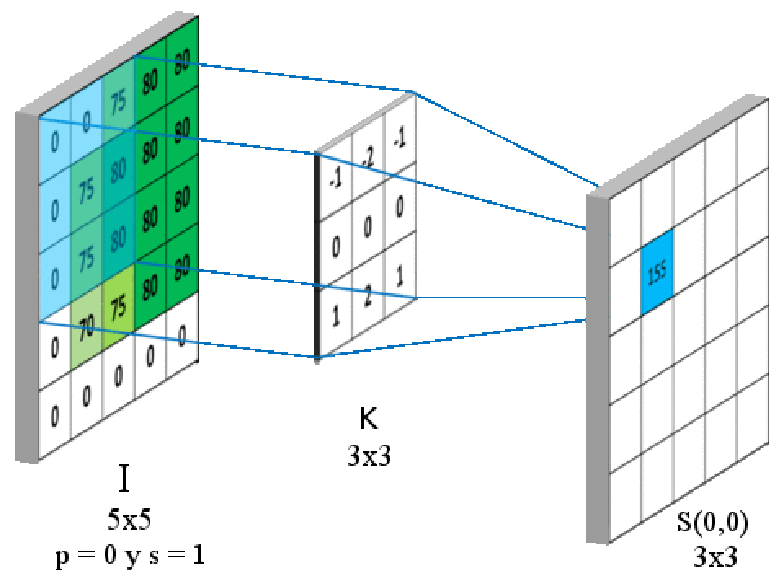
\includegraphics[width=1\linewidth]{2_CAPITULO0/IMG/padding1.png}
                        \begin{justify}
                            \textit{Nota.} La operación genera una matriz de salida de 3x3 donde, por ejemplo, S(0,0) tiene un valor de 155 después de la convolución; la matriz resultante es dos unidades menor que la original por no usar padding. Adaptado de \textcite{Goodfellow2016}.
                        \end{justify}                    
                        \label{padding1}
                    \end{figure}
                    
                    \begin{figure}[H] 
                        \caption{\doublespacing \\ \textit{ Cálculo de la convolución para la posición \( S(0, 1) \) en la matriz de salida.}} 
                        \centering
                        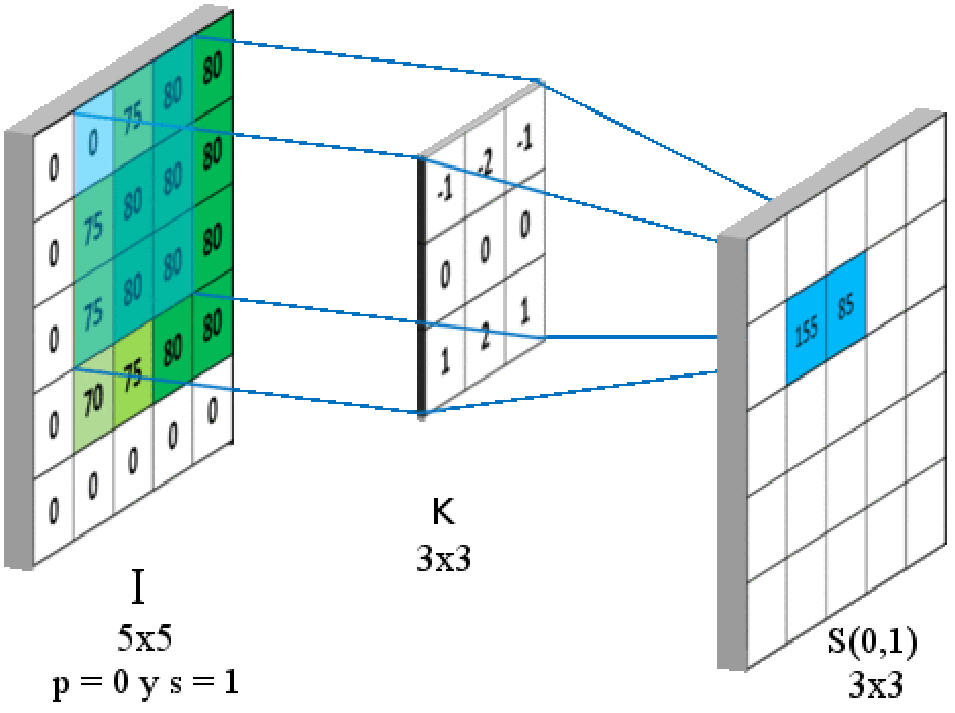
\includegraphics[width=1\linewidth]{2_CAPITULO0/IMG/padding2.png}
                        \begin{justify}
                            \textit{Nota.} La convolución involucra una matriz \(5 \times 5\) y un kernel \(3 \times 3\), resultando en \(S(0,1) = 85\), con líneas azules que representan la transformación. Adaptado de \textcite{Goodfellow2016}.
                        \end{justify}                    
                        \label{padding2}
                    \end{figure}
                    

                    En la mayoría de los casos, \( p = 0 \), pero si \( p > 0 \), la dimensión de la matriz de salida se calcula como:
                    
                    \begin{equation}
                        \text{Dimensión de Salida} = n + 2 \cdot p - f + 1 \times n + 2 \cdot p - f + 1
                    \end{equation}
                    
                    donde \( n \) es la dimensión de la matriz de entrada y \( f \) es la dimensión del filtro.
                    
                    Por ejemplo, en la \autoref{padding3}, considerando un padding \( p = 1 \), una matriz de entrada \( I \) de dimensiones \( 5 \times 5 \), y un filtro de dimensiones \( 3 \times 3 \), la matriz de salida resultante tendrá dimensiones \( 5 \times 5 \), manteniendo así la dimensión espacial de la matriz de entrada.

    
                    \begin{figure}[H] 
                        \caption{\doublespacing \\ \textit{Cálculo de la convolución de una matriz de entrada \( 5 \times 5 \) con un kernel \( 3 \times 3 \) con \( p = 1 \) y \( s = 1 \)}} 
                        \centering
                        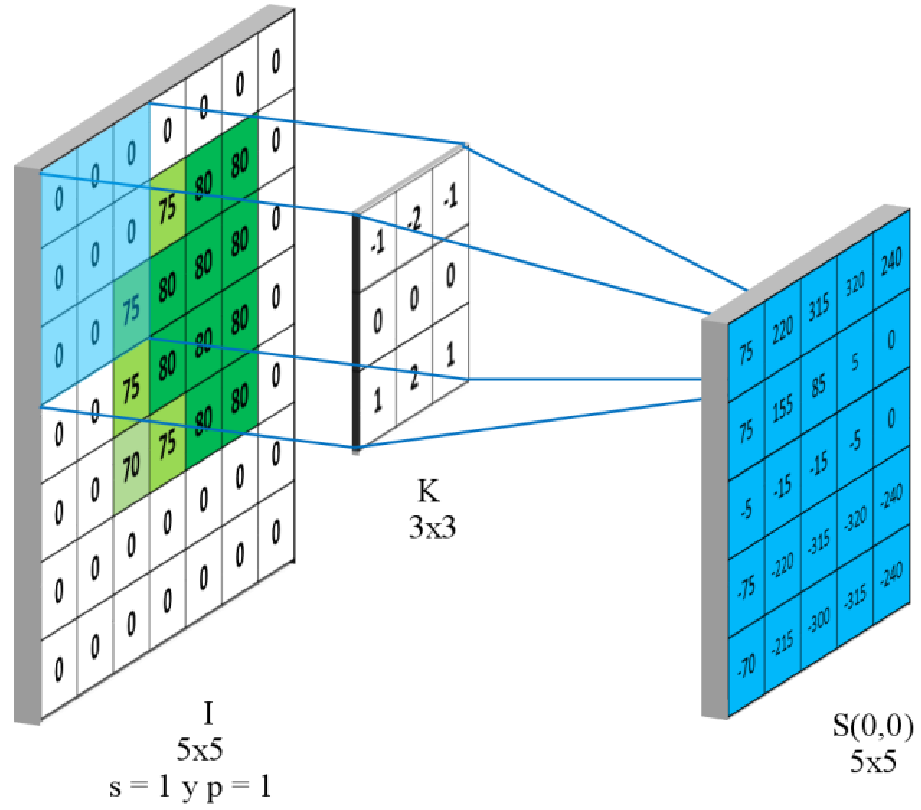
\includegraphics[width=1\linewidth]{2_CAPITULO0/IMG/padding3.png}
                        \begin{justify}
                            \textit{Nota.} \textit{Padding} de \( p=1 \) mantiene dimensiones de la imagen original, esencial para que redes neuronales aprendan patrones locales eficientemente. Adaptado de \textcite{Goodfellow2016}.
                        \end{justify}                    
                        \label{padding3}
                    \end{figure}

                    Las convoluciones pueden clasificarse en:
                    
                    \begin{itemize}
                        \item[-] \textbf{Convoluciones válidas:} No utilizan padding, resultando en una matriz de salida de dimensiones menores.
                        \item[-] \textbf{Convoluciones iguales:} Utilizan padding para asegurar que la matriz de salida tenga las mismas dimensiones que la matriz de entrada.
                    \end{itemize}
                    
                \paragraph{Stride}
                    Anteriormente ha sido denotado como \( s \), representa la cantidad de píxeles que el filtro se moverá durante la operación de convolución. Actualizando la fórmula de la dimensión de salida para incluir el stride, tenemos:
                    
                    \begin{equation}
                        \text{Dimensión de Salida} = \left\lfloor \frac{n + 2 \cdot p - f}{s} + 1 \right\rfloor \times \left\lfloor \frac{n + 2 \cdot p - f}{s} + 1 \right\rfloor
                    \end{equation}
                    
                    Por ejemplo, en la \autoref{stride}, con un stride \( s = 2 \), un padding \( p = 1 \), una matriz de entrada \( I \) de dimensiones \( 5 \times 5 \), y un filtro de dimensiones \( 3 \times 3 \), la matriz de salida resultante tendrá dimensiones \( 3 \times 3 \).
                    
                    \begin{figure}[H] 
                        \caption{\doublespacing \\ \textit{Convolución 2D con Padding de 1 y Stride de 2 en la Posición S(1, 1).}} 
                        \centering
                        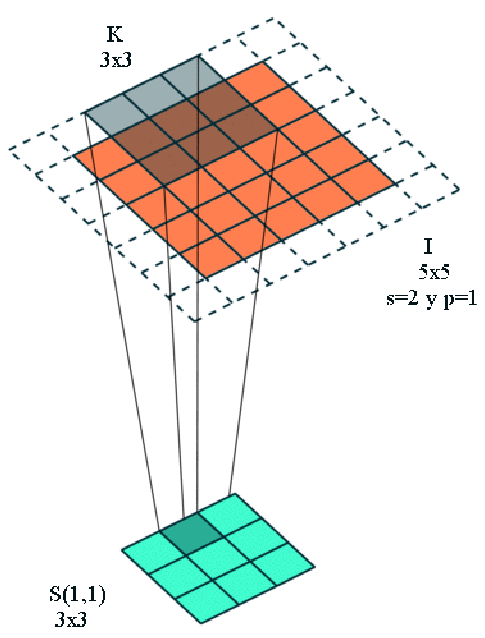
\includegraphics[width=0.8\linewidth]{2_CAPITULO0/IMG/stride.png}
                        \begin{justify}
                            \textit{Nota.} Convolución con stride de 2 y filtro de \(3 \times 3\), desplazando dos píxeles a la vez y padding que preserva información en bordes. Adaptado de \textcite{Goodfellow2016}.
                        \end{justify}                    
                        \label{stride}
                    \end{figure}
                    

            \subsubsection{Tipos de capas en una red neuronal convolucional}
                Las Redes Neuronales Convolucionales emplean una serie de capas específicas que incluyen: Capa de Entrada, Capa Convolucional, Capa de Agrupación, Capa Totalmente Conectada y Capa de Salida. Cada capa tiene funciones específicas y contribuye al rendimiento general de la red.
                \begin{figure}[H] 
                    \caption{\doublespacing \\ \textit{Representación esquemática de una Red Neuronal Convolucional.}} 
                    \centering
                    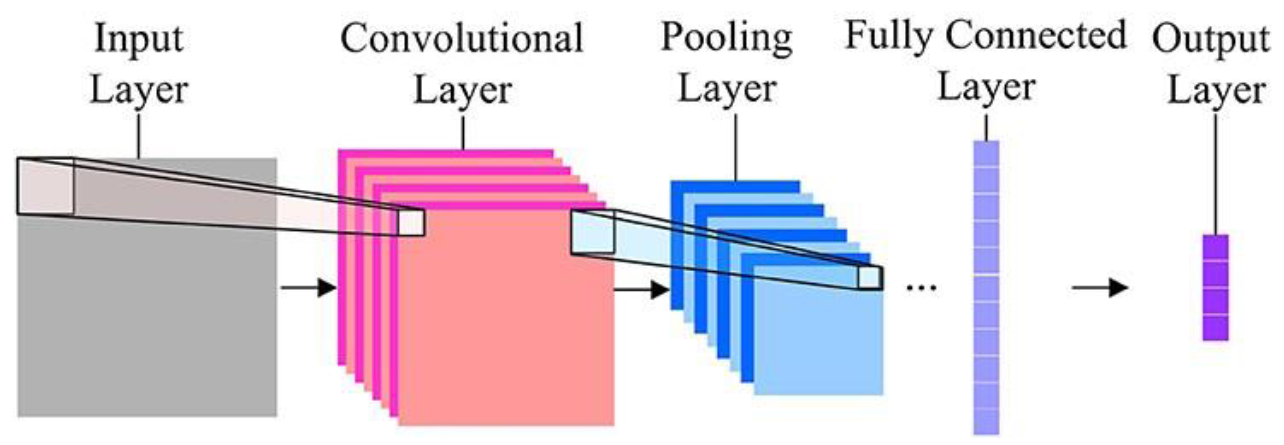
\includegraphics[width=1\linewidth]{2_CAPITULO0//IMG/tipos_capas.png}
                    \begin{justify}
                        \textit{Nota.} La estructura CNN: capas convolucionales detectan patrones y reducen tamaño; una capa conectada integra rasgos para la clasificación final, crucial en procesamiento visual. Adaptado de \textcite{Goodfellow2016}.
                    \end{justify}                    
                    \label{tipos_capas}
                \end{figure}
            
                
                \paragraph{Capa de Convolución}
                    Esta capa realiza operaciones de convolución en la entrada utilizando varios \textit{kernels}. Posteriormente, se agrega un sesgo al resultado y se pasa por una función de activación no lineal como ReLU. Esta función introduce no linealidad tras realizar operaciones lineales en las capas convolucionales. Aunque en el pasado se usaron funciones como tanh y sigmoid, ReLU ha demostrado ser más eficiente en términos de tiempo de entrenamiento y precisión.
                    
                    \begin{figure}[H] 
                        \caption{\doublespacing \\ \textit{Función de activación ReLU.}} 
                        \centering
                        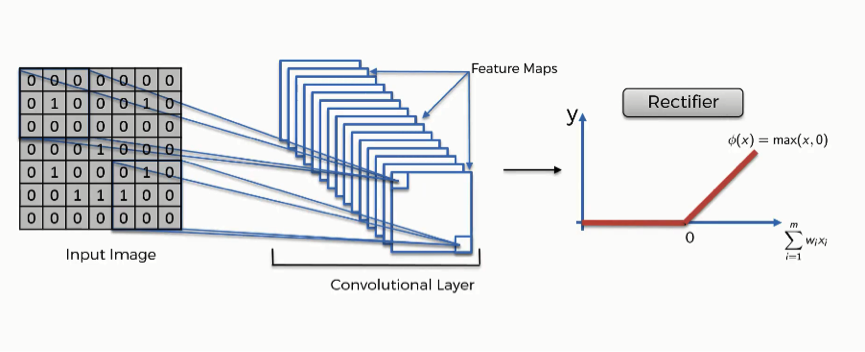
\includegraphics[width=1\linewidth]{2_CAPITULO0//IMG/relu.png}
                        \begin{justify}
                            \textit{Nota.} La función ReLU introduce no linealidad, ayudando a la red a capturar patrones complejos y optimizando el entrenamiento y precisión, evidenciando su ventaja sobre funciones previas como tanh o sigmoid. Tomado de \textcite{Kalita2022}.
                        \end{justify}                    
                        \label{relu}
                    \end{figure}
                
                \paragraph{Capa de agrupación}
                    Destinada a reducir las dimensiones de la entrada, la Capa de Agrupación mejora la eficiencia y robustez de la red. Una técnica popular aquí es el \textit{Max Pooling}, que selecciona el valor máximo de un conjunto específico, en la \autoref{max_pooling} se muestra un ejemplo donde una matriz I de tamaño 6 x 6, con un s igual a 3 y p igual a 0 . Esto es especialmente útil porque no introduce parámetros adicionales y es computacionalmente eficiente.
                    
                    Diversas técnicas de agrupación incluyen:
                    
                    \begin{itemize}
                        \item[-] Agrupación Máxima: \( s_j = \max_{i \in R_j} a_i \)
                        \item[-] Agrupación Promedio: \( s_j = \frac{1}{|R_j|} \sum_{i \in R_j} a_i \)
                        \item[-] Agrupación Estocástica: \( p_j = \frac{a_i}{\sum_{k \in R_j} a_k} \)
                    \end{itemize}

                    \begin{figure}[H] 
                        \caption{\doublespacing \\ \textit{Max-Pooling con padding de 0 y stride de 3 en posición S(0, 0).}} 
                        \centering
                        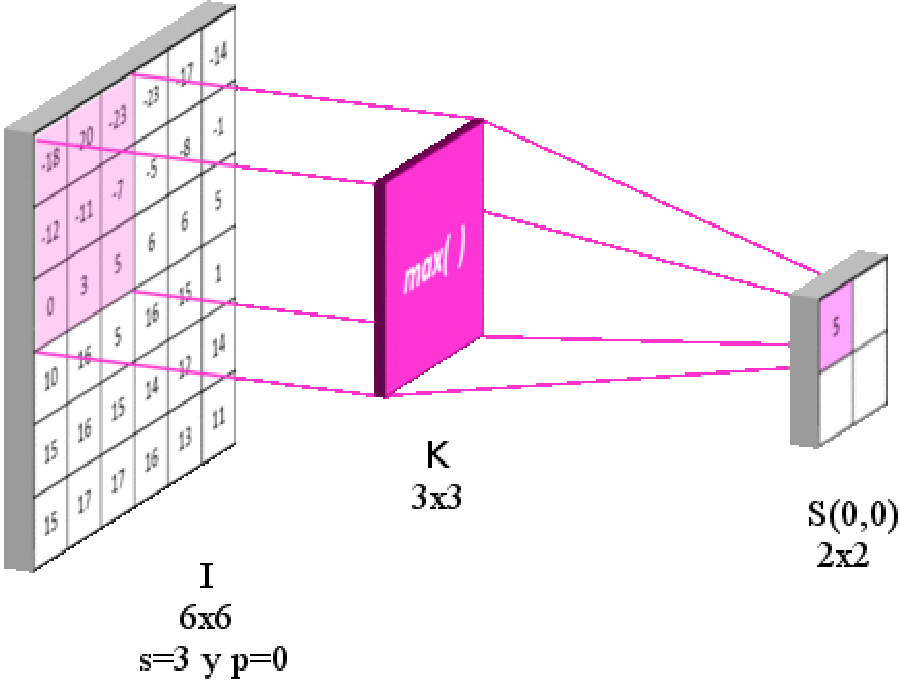
\includegraphics[width=1\linewidth]{2_CAPITULO0//IMG/max_pooling.png}
                        \begin{justify}
                            \textit{Nota.} Max-Pooling con kernel de \(3 \times 3\) y stride de 3 sobre una matriz \(6 \times 6\) extrae máximos locales, resultando en una matriz \(2 \times 2\), compactando información y resaltando características prominentes sin pérdida significativa. Adaptado de \textcite{Goodfellow2016}.
                        \end{justify}                    
                        \label{max_pooling}
                    \end{figure}
                

                \paragraph{Capa totalmente conectada}
                    Después de la agrupación, la entrada se pasa a una capa totalmente conectada que la conecta con la capa de salida, estableciendo conexiones entre todas las unidades \autocite{Goodfellow2016}.
                
                \paragraph{Hiperparámetros}
                    Los hiperparámetros, a diferencia de los parámetros, son valores preestablecidos que determinan cómo se comporta un algoritmo durante el entrenamiento. Estos se definen antes del proceso de aprendizaje y no se adaptan automáticamente durante el mismo \autocite{Goodfellow2016}.
                    
                    Al diseñar arquitecturas de Redes Neuronales Convolucionales (CNN), se consideran diversos hiperparámetros, entre los cuales se encuentran:
                    
                    \begin{itemize}
                        \item[-] \textbf{Tamaño del kernel:} Definido por la dimensión \( f \times f \), se utiliza en la capa convolucional o de agrupación.
                        \item[-] \textbf{Padding:} Indica cuántos píxeles se añaden alrededor de la imagen, normalmente rellenos con cero, para ajustar las dimensiones durante las convoluciones.
                        \item[-] \textbf{Stride:} Define cuántos píxeles se desplaza el kernel durante la convolución.
                        \item[-] \textbf{Número de kernels:} La cantidad de filtros en una capa convolucional.
                        \item[-] \textbf{Número de capas:} El total de capas en una CNN.
                        \item[-] \textbf{Función de activación:} Función no lineal aplicada tras la convolución, comúnmente ReLU, Sigmoid o Tanh.
                    \end{itemize}
                    
                    También se deben considerar hiperparámetros específicos al definir el conjunto de entrenamiento:
                    
                    \begin{itemize}
                        \item[-] \textbf{Muestras de entrenamiento:} Total de ejemplos utilizados en el entrenamiento.
                        \item[-] \textbf{Tamaño del lote (batch size):} Número de ejemplos procesados en una sola iteración de entrenamiento.
                        \item[-] \textbf{Iteraciones:} Total de lotes necesarios para completar una época.
                        \item[-] \textbf{Épocas:} Número de veces que se procesa el conjunto completo de entrenamiento.
                        \item[-] \textbf{Tasa de aprendizaje (\( \varepsilon \)):} Define la magnitud de ajuste de los pesos en función del gradiente de pérdida.
                    \end{itemize}
                    
                    El número de épocas se calcula según la relación:
                    
                    \begin{equation}
                        \text{epochs} = \frac{\text{batch\_size} \times \text{iterations}}{\text{training\_samples}}
                    \end{equation}
                    
                    Existen otros hiperparámetros que se emplean como métodos de regularización:
                    
                    \begin{itemize}
                        \item[-] \textbf{Regularización L2:} Penaliza la magnitud de los pesos para evitar sobreajuste.
                        \item[-] \textbf{Regularización L1:} Similar a L2, pero puede hacer que algunos pesos sean exactamente cero.
                        \item[-] \textbf{Dropout:} Durante el entrenamiento, desactiva aleatoriamente algunas neuronas para prevenir la dependencia excesiva en cualquier neurona individual.
                        \item[-] \textbf{Augmentation:} Amplía el conjunto de entrenamiento al introducir variaciones menores, como rotaciones y escalas, para mejorar la generalización del modelo.
                    \end{itemize}

        \section{Definición de términos}
                       
            \subsection{Armonización de datos}
                Se refiere al proceso de ajustar conjuntos de datos para que sean consistentes entre sí en términos de escala, resolución, calibración y geometría. En la teledetección, la armonización es clave para comparar y analizar imágenes tomadas por diferentes sensores o tecnologías a lo largo del tiempo, como las de las distintas generaciones del sensor Landsat MSS.
                
            \subsection{BRDF (Bidirectional Reflectance Distribution Function)}
                Función que describe cómo la reflectancia de una superficie varía con la geometría de la iluminación y la observación. Es esencial para la corrección y normalización de imágenes satelitales, permitiendo comparaciones más precisas entre diferentes fechas y condiciones de iluminación.
            
            \subsection{CNN (Redes Neuronales Convolucionales)}
                Tipo de red neuronal diseñada para procesar datos con una estructura de grilla, como imágenes, utilizando convoluciones para extraer características relevantes. Son ampliamente utilizadas en la teledetección para tareas como la segmentación de imágenes y la clasificación de objetos.
            
            \subsection{Co-registración}
                Proceso de alinear geométricamente varias imágenes de diferentes sensores para que coincidan espacialmente. Es esencial para el análisis multitemporal y la fusión de imágenes, permitiendo comparaciones precisas y la integración de datos de diversas fuentes.
            
            \subsection{Cubo de datos}
                En el contexto de la teledetección y la ciencia de la Tierra, un cubo de datos se refiere a una colección multidimensional de datos que se ha estructurado de tal manera que permite un análisis eficiente y flexible. Los cubos de datos generalmente organizan la información en tres dimensiones: espacial (latitud y longitud), temporal (tiempo) y espectral (bandas de captura del sensor), lo que facilita diversas operaciones analíticas como la comparación temporal y el análisis de cambios.
            
            \subsection{Deep learning}
                Es una rama del aprendizaje automático basada en algoritmos que modelan abstracciones de alto nivel en datos usando arquitecturas compuestas de múltiples transformaciones no lineales. En el contexto de la teledetección, se utiliza para interpretar y procesar grandes volúmenes de datos de imágenes satelitales, permitiendo la identificación de patrones y la realización de tareas como la clasificación de la cobertura terrestre y la detección de cambios.
            
            \subsection{Entornos conda}
                Conda es un sistema de gestión de paquetes y entornos que permite a los usuarios instalar y gestionar bibliotecas y dependencias en múltiples lenguajes de programación, como Python y R. Los entornos Conda permiten aislar diferentes proyectos y sus dependencias, evitando conflictos entre bibliotecas y facilitando la reproducibilidad de los experimentos. Son particularmente útiles en la teledetección y el procesamiento de imágenes, donde diferentes proyectos pueden requerir versiones específicas de librerías como TensorFlow, PyTorch, GDAL, y otras herramientas de análisis y visualización de datos.
                

            \subsection{ESRCNN (Extended Super-Resolution Convolutional Neural Network)}
                Modelo de red neuronal utilizado para mejorar la resolución espacial de imágenes satelitales mediante la fusión de datos de diferentes fuentes. Este modelo ha demostrado ser eficaz en la producción de imágenes coherentes y de alta calidad a partir de datos de menor resolución.
            
            \subsection{GAN (Generative Adversarial Network)}
                Tipo de red neuronal que consiste en dos modelos en competencia, un generador y un discriminador, utilizada para generar datos sintéticos que parecen reales. Es particularmente útil en la generación de imágenes de alta resolución y en la simulación de datos faltantes.
            
            \subsection{Generación de banda virtual}
                En la teledetección, la generación de bandas virtuales implica la creación de nuevas bandas de datos que no se capturan directamente por el sensor, generalmente a través de algoritmos que simulan estas bandas basándose en las bandas existentes y las relaciones conocidas entre ellas. Esto puede ayudar a mejorar la interpretación y análisis de las imágenes, especialmente cuando se combinan datos de diferentes sensores que tienen distintas capacidades espectrales.
            
            \subsection{Histogram matching}
                Es una técnica de procesamiento de imágenes que se utiliza para ajustar la distribución de brillo de una imagen para que coincida con la distribución de otra imagen. Esto se utiliza en la armonización de imágenes de diferentes sensores para que las características similares tengan una apariencia similar en términos de intensidad y contraste.
            
            \subsection{Landsat}
                Serie de satélites de observación terrestre gestionados por la NASA y el USGS, utilizados para monitorear y estudiar la superficie de la Tierra desde 1972. Proporcionan datos esenciales para investigaciones en áreas como la agricultura, la silvicultura, y el monitoreo ambiental.
                
            \subsection{MSS (Multi-Spectral Scanner)}
                Primer sensor utilizado en los satélites Landsat 1 a 5, que captura imágenes en varias bandas espectrales con una resolución espacial específica. Este sensor ha sido crucial para el estudio de cambios en la superficie terrestre a lo largo de varias décadas.
                
            \subsection{NDVI}
                Índice utilizado para evaluar la presencia y condición de la vegetación en la superficie terrestre, calculado a partir de las bandas espectrales del rojo y el infrarrojo cercano. Es una herramienta crucial para el monitoreo de la salud de los ecosistemas y la gestión de recursos agrícolas.
            
            \subsection{Segmentación de imágenes}
                Técnica de procesamiento de imágenes que divide una imagen en regiones o segmentos distintos para facilitar su análisis y procesamiento posterior. Es fundamental en la teledetección para la identificación y clasificación de diferentes tipos de cobertura terrestre.
            
            \subsection{Super-resolución}
                Técnica para aumentar la resolución de imágenes utilizando algoritmos avanzados, como redes neuronales, para generar detalles adicionales a partir de datos de baja resolución. Esto mejora la calidad y la utilidad de las imágenes satelitales para análisis detallados.
            
            \subsection{TM (Thematic Mapper)}
                Sensor avanzado utilizado en los satélites Landsat 4 y 5 que ofrece mejoras en la resolución espacial y espectral en comparación con el MSS. Es capaz de capturar imágenes en siete bandas espectrales, permitiendo análisis más detallados y precisos.
            
            \subsection{Transformadas de Fourier}
                En el procesamiento de imágenes, la transformada de Fourier es una herramienta matemática que descompone una imagen en sus frecuencias espaciales. Esto es útil para analizar patrones periódicos y filtrar ruido o para operaciones de corrección geométrica y espectral en el dominio de la frecuencia.
            